% Options for packages loaded elsewhere
\PassOptionsToPackage{unicode}{hyperref}
\PassOptionsToPackage{hyphens}{url}
%
\documentclass[
]{book}
\usepackage{lmodern}
\usepackage{amssymb,amsmath}
\usepackage{ifxetex,ifluatex}
\ifnum 0\ifxetex 1\fi\ifluatex 1\fi=0 % if pdftex
  \usepackage[T1]{fontenc}
  \usepackage[utf8]{inputenc}
  \usepackage{textcomp} % provide euro and other symbols
\else % if luatex or xetex
  \usepackage{unicode-math}
  \defaultfontfeatures{Scale=MatchLowercase}
  \defaultfontfeatures[\rmfamily]{Ligatures=TeX,Scale=1}
\fi
% Use upquote if available, for straight quotes in verbatim environments
\IfFileExists{upquote.sty}{\usepackage{upquote}}{}
\IfFileExists{microtype.sty}{% use microtype if available
  \usepackage[]{microtype}
  \UseMicrotypeSet[protrusion]{basicmath} % disable protrusion for tt fonts
}{}
\makeatletter
\@ifundefined{KOMAClassName}{% if non-KOMA class
  \IfFileExists{parskip.sty}{%
    \usepackage{parskip}
  }{% else
    \setlength{\parindent}{0pt}
    \setlength{\parskip}{6pt plus 2pt minus 1pt}}
}{% if KOMA class
  \KOMAoptions{parskip=half}}
\makeatother
\usepackage{xcolor}
\IfFileExists{xurl.sty}{\usepackage{xurl}}{} % add URL line breaks if available
\IfFileExists{bookmark.sty}{\usepackage{bookmark}}{\usepackage{hyperref}}
\hypersetup{
  pdftitle={Eagle I.O Consultant Manual},
  pdfauthor={Eagle I.O},
  hidelinks,
  pdfcreator={LaTeX via pandoc}}
\urlstyle{same} % disable monospaced font for URLs
\usepackage{longtable,booktabs}
% Correct order of tables after \paragraph or \subparagraph
\usepackage{etoolbox}
\makeatletter
\patchcmd\longtable{\par}{\if@noskipsec\mbox{}\fi\par}{}{}
\makeatother
% Allow footnotes in longtable head/foot
\IfFileExists{footnotehyper.sty}{\usepackage{footnotehyper}}{\usepackage{footnote}}
\makesavenoteenv{longtable}
\usepackage{graphicx,grffile}
\makeatletter
\def\maxwidth{\ifdim\Gin@nat@width>\linewidth\linewidth\else\Gin@nat@width\fi}
\def\maxheight{\ifdim\Gin@nat@height>\textheight\textheight\else\Gin@nat@height\fi}
\makeatother
% Scale images if necessary, so that they will not overflow the page
% margins by default, and it is still possible to overwrite the defaults
% using explicit options in \includegraphics[width, height, ...]{}
\setkeys{Gin}{width=\maxwidth,height=\maxheight,keepaspectratio}
% Set default figure placement to htbp
\makeatletter
\def\fps@figure{htbp}
\makeatother
\setlength{\emergencystretch}{3em} % prevent overfull lines
\providecommand{\tightlist}{%
  \setlength{\itemsep}{0pt}\setlength{\parskip}{0pt}}
\setcounter{secnumdepth}{5}
\usepackage{booktabs}
\usepackage[]{natbib}
\bibliographystyle{apalike}

\title{Eagle I.O Consultant Manual}
\author{Eagle I.O}
\date{Most recently updated Sunday June 07 2020 8:58:37 PM Eastern}

\begin{document}
\maketitle

{
\setcounter{tocdepth}{1}
\tableofcontents
}
\#Homepage \{-\#homepage\}


\includegraphics{images/eagleio.PNG}

This is the student consultant handbook for members of Eagle I.O. Herein lie expectations, responsibilities, and strategy to keep Eagle I.O viable with future \href{https://www.montclair.edu/psychology/graduate-programs/industrial-organizational-psychology/}{Montclair State University I/O Psychology} cohorts\ldots{}

\hypertarget{introduction}{%
\chapter{Introduction}\label{introduction}}

\begin{itemize}
\tightlist
\item
  This is the consultant manual for Eagle I.O student consultants. It contains the expectations, roles, and responsibilities of MSU student consultants who are members of Eagle I.O.
\item
  As of Spring semester 2020, the ongoing projects for Eagle I.O. include: 1) a mentorship program between the 1 year and 2nd year cohorts, 2) an engagement survey, and 3) this student consultant manual (which includes, for example, a succession plan to sustain and grow Eagle I.O)
\item
  Future aspirations are to have Eagle I.O. be a client-facing organization that can provide student-led solutions to external clients
\end{itemize}

\hypertarget{intro}{%
\chapter{Duties}\label{intro}}

\hypertarget{eagle-i.o-expectations}{%
\section{Eagle I.O Expectations}\label{eagle-i.o-expectations}}

\begin{itemize}
\tightlist
\item
  Attend mandatory bi-weekly meetings (or monthly?)
\item
  Contribute to Eagle I.O projects (mentorship program, survey developments)
\item
  Be able to read and respond to emails pertaining to Eagle I-O/Mentor Program in a timely manner (?Move this responsibility to Mentor Program Coordinator?)
\item
  Attend Eagle I-O events (METRO, social meetings, mentor meetings)
\item
  Be a professional ambassador (aligned with: 1) Eagle, 2) MSU, and 3) the larger discipline of I-O Psychology)
\end{itemize}

\hypertarget{eagle-i.o-requirements-ksas}{%
\section{Eagle I.O Requirements (KSA's)}\label{eagle-i.o-requirements-ksas}}

\begin{itemize}
\tightlist
\item
  Ability to work in a team-based environment
\item
  Be receptive to group members opinions and suggestions
\item
  Collaborate with group members to facilitate growth in current and future projects
\item
  Update Handbooks to support growth of program for future cohorts
\end{itemize}

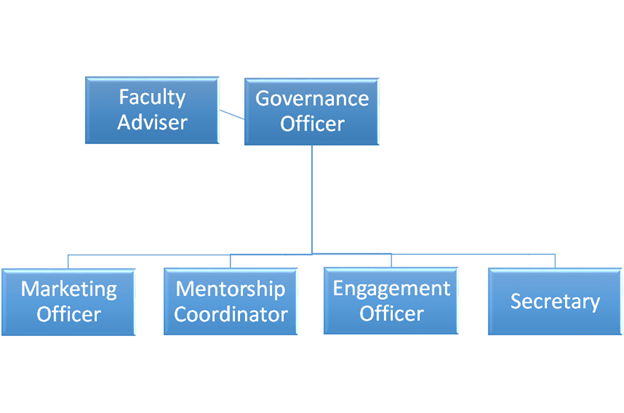
\includegraphics{images/orgchart.PNG}

\hypertarget{responsibilities}{%
\chapter{Responsibilities}\label{responsibilities}}

These individuals function as team leads - they are responsible for the bulleted information, but they are expected to execute tasks within teams:

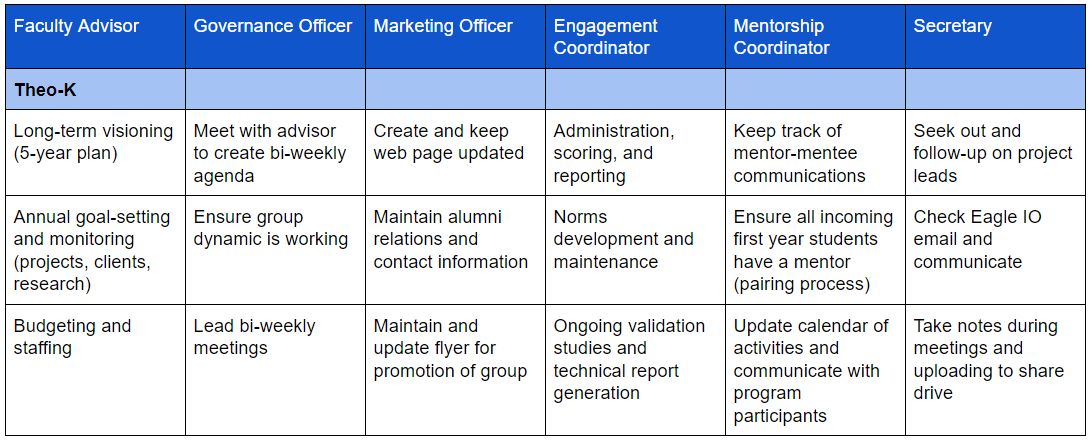
\includegraphics{images/roles.PNG}

\hypertarget{governance}{%
\chapter{Governance}\label{governance}}

\hypertarget{meetings}{%
\section{Meetings}\label{meetings}}

\begin{itemize}
\tightlist
\item
  Time requirements of Eagle IO members

  \begin{itemize}
  \tightlist
  \item
    Necessary \# of meetings: attend every meeting {[}miss only one{]}

    \begin{itemize}
    \tightlist
    \item
      If missing more than one meeting, then try calling in or provide a valid reason.
    \end{itemize}
  \item
    Keeping track of the inbox on your assigned week
  \end{itemize}
\end{itemize}

\hypertarget{mentorship-program-management}{%
\section{Mentorship Program Management}\label{mentorship-program-management}}

\begin{itemize}
\tightlist
\item
  How to match mentors and mentees (depending on the success of this semester) consider the method used to match or if other things should be considered.

  \begin{itemize}
  \tightlist
  \item
    Form a survey team to create a qualtrics and do the matching process
  \item
    Consolidate questions (5): name, hometown, undergrad major/minor, part/full time, and academic/applied
  \end{itemize}
\item
  Duration or partnership between mentee and mentor (semester or annual)

  \begin{itemize}
  \tightlist
  \item
    Mandatory to keep them mentor/mentee partnership for a semester

    \begin{itemize}
    \tightlist
    \item
      Ask them if they want to keep the formal relationship and/or opt out and be a mentor themselves
    \end{itemize}
  \end{itemize}
\item
  Involvement of professors in mentor program beyond Dr.~Kulas and Dr.~Dan

  \begin{itemize}
  \tightlist
  \item
    Meetings between mentors and mentees at least 3

    \begin{itemize}
    \tightlist
    \item
      Meeting 1: Individual Development Plan
    \item
      Meeting 2: I/O related event
    \item
      Meeting 3: formal/informal event
    \end{itemize}
  \end{itemize}
\end{itemize}

\hypertarget{consultant-development-plan}{%
\section{Consultant Development Plan}\label{consultant-development-plan}}

\begin{itemize}
\tightlist
\item
  Either have each consultant discuss and fill out their own individual development plan in terms of Eagle I.O. or have a development (filled out together) for the organization

  \begin{itemize}
  \tightlist
  \item
    Potential skills: professional, technical, or R-related skills
  \end{itemize}
\end{itemize}

Share the Organization's Structure: All students are required to write and submit a constitution. \href{https://www.utdallas.edu/soc/manual/04/\#leadership}{See Chapter Two for sample constitution}

\begin{itemize}
\tightlist
\item
  Constitution and by-laws
\item
  Job descriptions/role classifications
\item
  Organizational goals and objectives
\item
  Status reports on ongoing projects
\item
  Evaluation of previous projects and programs
\item
  Resources and contact lists
\item
  Mailing lists
\item
  Historical records, scrapbooks, and equipment
\end{itemize}

\hypertarget{succession-planning}{%
\chapter{Succession Planning}\label{succession-planning}}

\begin{itemize}
\tightlist
\item
  Framework:

  \begin{itemize}
  \tightlist
  \item
    Lens to get new mentees
  \item
    Recruitment and selection
  \item
    Identify possible Eagle IO members
  \end{itemize}
\end{itemize}

Criteria:

\begin{itemize}
\tightlist
\item
  Process:

  \begin{itemize}
  \tightlist
  \item
    Role assignments will be discussed after first years have shadowed for a semester (shadowing occurs Spring semester)

    \begin{itemize}
    \tightlist
    \item
      Shadowing = come to meetings
    \end{itemize}
  \end{itemize}
\end{itemize}

Timeline

Actions

Outcomes

Deliverables

November of 3rd Semester

Eagle IO will send out to current first years an invitation to become part of the the group

Get an estimate of how many students are interested in joining Eagle IO

Email invitation

December of 3rd Semester

Determine how many first year students are interested in joining Eagle IO

Select best candidates based on criteria to join

Criteria to join: GPA above 3.5, Applied/academic experience (i.e.~internship, research), Attend I/O related event (i.e.~Metro, SIOP, Eagle IO events)

January of 4th Semester

Send out email to people selected to join Eagle IO

Finalize how many people will be joining the group

Agenda for first meeting with new Eagle IO students

February of 4th Semester

Have first meeting with new Eagle IO students

Onboarding: The purpose of this meeting will be to a) exmplain expectations of members, b) provide guidelines as a member and mentor, and c) get a sense of the roles that are available and what new members are interested in

The purpose of the meeting should include presenting current projects to first year students and set dates for future meetings that allow all new members to attend, and plan agenda for next meeting.

April of 4th Semester

Last Eagle IO meeting for the year: Conclude succession plan

Select students to be placed intheir new roles as part of Eagle IO, and communicate oprogress on products and governance

Role fulfillment for Eagle IO and ensuring new members have access to Eagle IO documents/projects

  \bibliography{book.bib,packages.bib}

\end{document}
